\section{Endogenous Reputation Concerns} \label{sec:endogenous}
This section shows that the quadratic form of the reputation benefit postulated in Section \ref{sec:Model} endogenously arises in a two-period model. Unless otherwise noted, the same assumptions as the baseline model prevail. We discuss economic implications drawn from the equilibrium analyses in Subsection \ref{ss:implications}.

%===========================================
\subsection{Setup} \label{sec:setupEndog}
There are two periods, $t=0,1$. In each period, the trader with skill $|s|$ picks an asset that yields a payoff $\delta_{t}\sim N(\hat{\delta}_{t}+s,\omega_{\delta})$ at the end of the period, where $\hat{\delta}_{t}$ is the market maker's prior expectation about $\delta_{t}$. Each asset lives only for one period. Although the trader picks different assets in $t=0$ and $t=1$, both of them are characterized by the same $s$ because $s$ represents her time-invariant skill. In other words, her skill allows her to {\it systematically} pick an asset such that the market maker's prior expectation about $\delta_{t}$ is biased by $|s|$. %this means that each trader has her own pool of assets to pick from; not sure this is clear from the formulation.
We assume that the market is anonymous, meaning that market makers cannot track which trader selects which assets, while the recruiter can. This assumption, combined with the existence of a continuum of traders with various $s$, implies that market makers at $t=1$ cannot update their estimate of each trader’s $s$, whereas the recruiter can.\footnote{This assumption is justified by the anonymity of the market. Each market maker trades with a different trader in each period and cannot track or identify which traders have traded which assets in the past. Hence, he cannot update traders' skills based on past information. Conversely, recruiters may keep track of traders via direct and individual communications.} This distinction is critical: it is the market makers' inability to update the estimate of $s$ that allows the recruiter---who can update it---to potentially make profits by recruiting traders.

\paragraph{\normalfont{\it{Timing.}}}
The model unfolds as follows. \vspace*{-0.2cm}
	\begin{enumerate}
		\item At the beginning of $t=0$, each trader draws $s$ independently from $N(0,\omega_{s})$, which is her private information. She selects an asset and submits market order $x_{0}$ to the market maker for that asset, and liquidity investors' demand $u_{0}\sim N(0,\omega_{u,0})$ is realized. The market maker sets a price using order-flow information, $p_{0}=\mathrm{E}\left[\delta_{0}|x_{0}+u_{0}\right]$.
		\item At the end of $t=0$, the asset's payoff $\delta_{0}$ is realized, and the trader earns the profit, $\pi_{0}=(\delta_{0}-p_{0})x_{0}$.
		\item At the beginning of $t=1$, each trader meets the recruiter with probability $\varphi$. The recruiter observes the past execution price ($p_{0}$) and the realized payoff ($\delta_{0}$) of the asset that the trader has picked in $t=0$. The trader's $x_{0}$ and $\pi_{0}$ are not disclosed. %Need more discussion: why the trader does not reveal eta directly?
  The recruiter updates his estimate of the trader's $s$, obtaining the posterior mean $\hat{s}=\mathrm{E}\left[s|p_{0},\delta_{0}\right]$. The recruiter then employs the trader for a competitive salary:
			\begin{equation}
				w=\mathrm{E}[\pi_{1}|p_{0},\delta_{0}],
			\end{equation}
		where $\pi_{1}=(\delta_{1}-p_{1})x_{1}$ is the trading profit in $t=1$. Note that $w$ is determined by the recruiter's expectation about $\pi_{1}$.\footnote{An implicit assumption is that the trader encounters a recruiter upon losing her current job. Consequently, she always accepts the salary offered. A trader might find herself in such a situation due to the closure of a trading desk or the discontinuation of a fund, as described by eFinancialCareers (“\href{https://www.efinancialcareers.com/news/2014/05/investment-banks-now-poaching-floundering-hedge-funds}{How Investment Banks are Now Poaching from Floundering Hedge Funds},'' May 2014). Also, parameter $\varphi$ can incorporate labor mobility in the finance industry. For example, non-compete clauses and garden leave may reduce $\varphi$.} This is why the trader cares about the recruiter's perception of her $|s|$, leading to the endogenous reputation benefit. With probability $1-\varphi$, the trader does not meet the recruiter and remains with her current employer.\footnote{Alternatively, we could introduce the following setting. In the current firm's compensation, the proportion $\alpha$ is paid as a fixed wage, and the remaining portion is paid based on performance, $\pi_{t}$, while the recruiter's firm pays the $\alpha'$ portion as the fixed wage. The fixed wage paid by the current firm, $\bar{w}$, is already fixed, so that the trader's expected utility is written as $\mathrm{E}\left[\alpha\bar{w} + (1-\alpha)\pi_{0} + (1-\varphi)(\alpha\bar{w} + (1-\alpha)\pi_{1}) + \varphi(\alpha' w + (1-\alpha')\pi_{1})\right]$. Appropriately scaling and rewriting the coefficients of this utility, we obtain a maximization problem virtually identical to equation (\ref{max0a}), which yields all the results presented in this section.}  The trader submits market order $x_{1}$ to the market maker. Liquidity investors' demand $u_{1}\sim N(0,\omega_{u,1})$ is realized ($\omega_{u,1}$ and $\omega_{u,0}$ can be different). The market maker sets the price $p_{1}=\mathrm{E}\left[\delta_{1}|x_{1}+u_{1}\right]$.
		\item At the end of $t=1$, $\delta_{1}$ is realized and $\pi_{1}$ is determined.
	\end{enumerate}
	The trader's problem at the beginning of $t=0$ is
	\begin{equation}
		\max_{x_{0}}\ \mathrm{E}\left[\pi_{0}+\varphi w+(1-\varphi)\pi_{1}|s\right].\label{max0a}
	\end{equation}


%\footnote{Alternatively, we could introduce the following setting. Both in the current firm and the recruiter's firm, the proportion $\alpha$ of the compensation is paid as a fixed wage, while the remaining portion is paid based on performance, $\pi_{t}$. The fixed wage in the current compensation is already fixed at some constant, $\bar{w}$, so that the recruiter's expected utility is written as $\mathrm{E}\left[\alpha\bar{w} + (1-\alpha)\pi_{0} + (1-\varphi)(\alpha\bar{w} + (1-\alpha)\pi_{0}) + \varphi(\alpha w + (1-\alpha)\pi_{1})\right]$. Appropriately scaling and rewriting the coefficients of this utility, we obtain the same result as presented in equation (\ref{max0a}).}

%[Y: I don't understand this footnote.]
%\footnote{We assume that a trader always accepts the competitive salary. For reasons outside the model, she has to sell her know-how. The trader's trading decisions are independent absent the $\varphi$-event, such that the results are the same whether we assume that the trader exits all financial markets or trades on her own account if not meeting a recruiter.}

%Figure \ref{fig:timeline} summarizes the timing of the two-period model.

%\bigskip
%\centerline{\bf [Place Figure~\ref{fig:timeline} about here]}
%\bigskip

%===========================================
\subsection{Equilibrium} \label{ss:eqm_endog}
%\textit{Definition} [\textbf{?}]%An equilibrium --- subperfect bayesian eqm? see how to define.

We first solve the problems in $t=1$ and obtain the salary, $w$, which is shown to be a quadratic function of the perceived skill, $|\hat{s}|$. Subsequently, we solve the problems in $t=0$, which are similar to those of Section \ref{sec:Model}.

%-------------------------------------------
\subsubsection{Period 1} \label{sss:period1}
In $t=1$, each trader has no reputation concerns. Hence, she simply chooses $x_{1}$ to maximize $\pi_{1}$, resulting in the standard \citet{kyle1985continuous} equilibrium.
\begin{lemma}[Equilibrium in $t=1$]\label{eqmPer1}
In $t=1$, each trader's trading strategy is characterized by $x_{1} =\beta_{1}s$, and the market maker sets the execution price according to $p_{1}=\hat{\delta}_{1}+\lambda_{1}\left(x_{1}+u_{1}\right)$, where $\beta_{1}\equiv\sqrt{\frac{\omega_{u,1}}{\omega_{s}}}$ and $\lambda_{1}\equiv\frac{1}{2}\sqrt{\frac{\omega_{s}}{\omega_{u,1}}}$.
\end{lemma}
Lemma \ref{eqmPer1} yields the trader's profit, $\pi_{1}$. Then, the \textit{recruiter's} expectation about $\pi_{1}$ determines the trader's salary when she meets the recruiter. 
\begin{lemma}[Trader's salary]\label{salary}
Let $\hat{s}$ and $\hat{\omega}_{s}$ be the posterior mean and variance of $s$ from the recruiter's point of view. The salary he offers to the trader is
\begin{equation}
w=\frac{\beta_{1}}{2}\left(\hat{s}^{2}+\hat{\omega}_{s}\right).\label{w}
\end{equation}
\end{lemma}
Lemma \ref{salary} gives the competitive wage, $w$, as a quadratic function of $\hat{s}$, providing a microfoundation for the reputation benefit assumed in Section \ref{sec:Model}. 

%-------------------------------------------
\subsubsection{Period 0} \label{sss:period0}
In $t=0$, the trader knows that she will potentially obtain $w$ in the form of \eqref{w}. Hence, plugging \eqref{w} into \eqref{max0a}, her objective function in $t=0$ is
\begin{equation}
\mathrm{E}\left[\pi_{0}+\frac{\varphi\beta_{1}}{2}\left(\hat{s}^{2}+\hat{\omega}_{s}\right)+(1-\varphi)\pi_{1}\Big|s\right].\label{max0a2}
\end{equation}
Since $\pi_{1}$ and $\hat{\omega}_{s}$ are independent of $x_{0}$, her optimization problem in $t=0$ is characterized by (\ref{max0b}) in the following proposition.

\begin{proposition}[Endogenous reputation]\label{prop:endogenous_reputation}
In $t=0$, each trader's maximization problem is identical to \eqref{max_prob} of Section \ref{sec:Model}, that is,
\begin{equation}
\max_{x_{0}}\mathrm{E}\left[\pi_{0}+\theta\hat{s}^{2}\big|s\right], \label{max0b}
\end{equation}
where parameter $\theta$ for reputation concerns is given by
\begin{equation}
 \theta\equiv\frac{\varphi}{2}\sqrt{\frac{\omega_{u,1}}{\omega_{s}}}. \label{eq:theta}
\end{equation}
\end{proposition}

Proposition \ref{prop:endogenous_reputation} provides a microfoundation to the quadratic form of the reputation benefit in Section \ref{sec:Model}. Moreover, $\theta$ is endogeneized as a composite parameter \eqref{eq:theta}. Not surprisingly, it is increasing in $\varphi$. It decreases with the trader's skill potential, $\omega_{s}$, suggesting that a high-potential trader is less concerned about her reputation. This is due to the {\it future} trading intensity $\beta_{1}$ and the price impact $\lambda_{1}$: a high-potential trader is likely to possess a high skill, which induces a large price impact in the future as well. Since it is difficult for the trader to exploit her skill in $t=1$, the competitive wage becomes less responsive to $|s|$, weakening the reputation concern.

As problem \eqref{max0b} is effectively the same as \eqref{max_prob}, the equilibrium outcomes resemble Proposition \ref{prop:eqm}. However, unlike Proposition \ref{prop:eqm}, the impact of the skill potential $\omega_{s}$ on the equilibrium characterization is generalized due to the dependence of $\theta$ on $\omega_{s}$. This is summarized by the following proposition, which is graphically presented in Figure \ref{fig:theta_end}.

\begin{proposition}[Equilibrium in $t=0$]\label{prop:endogenous}
The equilibrium at $t=0$ is characterized as follows.
\begin{enumerate}[topsep=2.5pt]
\item If $\varphi$ is large enough, there are two thresholds for the skill potential, denoted as $\ubar{\omega}_{s}>0$ and $\bar{\omega}_{s}$ $(\geq \ubar{\omega}_{s})$, such that
 \begin{enumerate}[topsep=2.5pt, label=(\roman*)]
\item for $\omega_{s} \geq \bar{\omega}_{s}$, the low-$\beta$ equilibrium is uniquely realized;
\item for $\omega_{s} \in (\ubar{\omega}_{s}, \bar{\omega}_{s})$, both the high- and low-$\beta$ equilibria arise;
\item for $\omega_{s} \leq \ubar{\omega}_{s}$, the high-$\beta$ equilibrium is uniquely realized.
\end{enumerate}
\item If $\varphi$ is small enough, there is a unique equilibrium. For small $\omega_{s}$, the high-$\beta$ equilibrium is realized, while for large $\omega_{s}$, the low-$\beta$ equilibrium is realized.
\end{enumerate}
\end{proposition}

%\begin{figure}[t]
\usetikzlibrary{decorations.pathreplacing}
%\tikzset{mynode/.style={inner sep=2pt,fill,outer sep=0,circle}}
\begin{center}
\hspace*{-2.2cm}
\begin{minipage}[b]{0.45\linewidth}
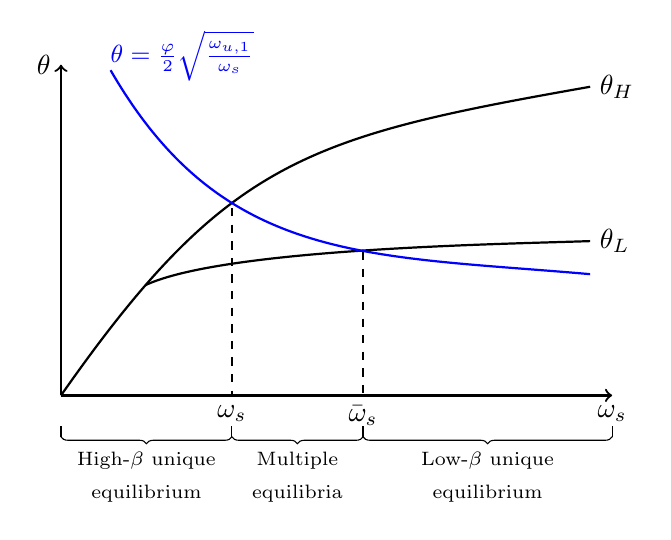
\begin{tikzpicture}[scale=1.4]

    \draw[thick,->] (0,0) -- (5,0) node[below] {$\omega_{s}$};
    \draw[thick,->] (0,0) -- (0,3) node[left] {$\theta$};
   
    % Curves
  
    \draw[thick] (0,0) to [out = 55, in = 190, looseness=1.2](4.8,2.8);
    \draw[thick] (0.765,1.) to [out = 25, in = 182, looseness=0.5](4.8,1.4);

    \node[fill=white, text=blue, inner sep=1pt] at (1.1, 3.08) {\small $\theta = \frac{\varphi}{2}\sqrt{\frac{\omega_{u,1}}{\omega_{s}}}$};
    
    \draw[thick, blue] (0.45, 2.95) to [out = 300, in = 175, looseness=1.1](4.8,1.1);

    % Points at the end of curves
    \node[right] at (4.8,2.8) {$\theta_H$};
    \node[right] at (4.8,1.4) {$\theta_L$};

    % Threshold for multiple eqm
    %\draw[thick,dashed] (0.77,1.) -- (0.765,0) node[below] {$\tilde{\omega}_{s}$};
    \draw[thick,dashed] (1.55, 1.7) -- (1.55,0.0) node[below] {$\ubar{\omega}_{s}$};%1.323
    \draw[thick,dashed] (2.74,1.3) -- (2.74,0.0) node[below] {$\bar{\omega}_{s}$};

    % Underbrace labels
    \draw[decorate,decoration={brace,mirror,raise=3pt}] (0,-0.3) -- (1.55,-0.3) node[midway,below=5pt, align=center] {\scriptsize High-$\beta$ unique\\ \scriptsize equilibrium};
    \draw (0,0.-0.28) -- (0,-0.38);
    \draw[decorate,decoration={brace,mirror,raise=3pt}] (1.55,-0.3) -- (2.74,-0.3) node[midway,below=5pt, align = center] {\scriptsize Multiple\\ \scriptsize equilibria};
    \draw (1.55,-0.28) -- (1.55,-0.38);
    \draw[decorate,decoration={brace,mirror,raise=3pt}] (2.74,-0.3) -- (5.0,-0.3) node[midway,below=5pt, align = center] {\scriptsize Low-$\beta$ unique\\ \scriptsize equilibrium};
    \draw (2.74,-0.28) -- (2.74, -0.38);
    \draw (5,-0.28) -- (5,-0.38);
    
\end{tikzpicture}
\end{minipage} \hspace{2.2cm}
\begin{minipage}[b]{0.45\linewidth}
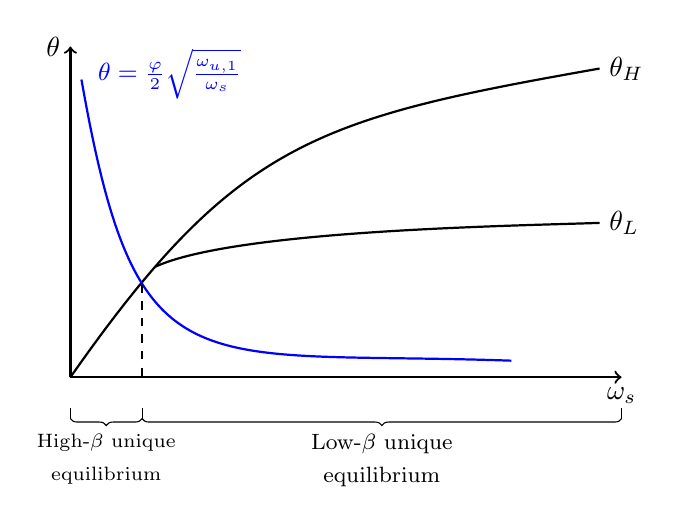
\begin{tikzpicture}[scale = 1.4]

% Axes
    \draw[thick,->] (0,0) -- (5,0) node[below] {$\omega_{s}$};
    \draw[thick,->] (0,0) -- (0,3) node[left] {$\theta$};
   
    % Curves
  
    \draw[thick] (0,0) to [out = 55, in = 190, looseness=1.2](4.8,2.8);
    \draw[thick] (0.765,1.) to [out = 25, in = 182, looseness=0.5](4.8,1.4);

    \node[fill=white, text=blue, inner sep=1pt] at (.9, 2.75) {\small $\theta = \frac{\varphi}{2}\sqrt{\frac{\omega_{u,1}}{\omega_{s}}}$};
    
    \draw[thick, blue] (0.1, 2.7) to [out = 280, in = 178, looseness=1.6](4.,0.15);

    % Points at the end of curves
    \node[right] at (4.8,2.8) {$\theta_H$};
    \node[right] at (4.8,1.4) {$\theta_L$};

    % Threshold for multiple eqm
    %\draw[thick,dashed] (0.77,1.) -- (0.765,0) node[below] {$\tilde{\omega}_{s}$};
    \draw[thick,dashed] (.65, .84) -- (.65,0.0);

    % Underbrace labels
    \draw[decorate,decoration={brace,mirror,raise=3pt}] (0,-0.3) -- (.65,-0.3) node[midway,below=5pt, align=center] {\scriptsize High-$\beta$ unique\\ \scriptsize equilibrium};
    \draw (0,0.-0.28) -- (0,-0.38);
    \draw[decorate,decoration={brace,mirror,raise=3pt}] (.65,-0.3) -- (5,-0.3) node[midway,below=5pt, align = center] {\footnotesize Low-$\beta$ unique\\ \footnotesize equilibrium};
    \draw (0.65,-0.28) -- (0.65,-0.38);
    \draw (5,-0.28) -- (5,-0.38);
\end{tikzpicture}
\end{minipage}
\end{center}
    \caption{Equilibrium Characterization with Endogenous $\theta$}
    \caption*{\footnotesize{Note: This figure illustrates the equilibrium states using the reputation concern, $\theta$, and the skill potential, $\omega_{s}$. The curves represented by $\theta_{H}$ and $\theta_{L}$ are identical to those in Figure \ref{fig:theta}} and Proposition \ref{prop:eqm}, while $\theta$ is endogenous and decreasing in $\omega_{s}$ as equation (\ref{eq:theta}) suggests.}
    \label{fig:theta_end}
\end{figure}\vspace*{0.2cm}
 \begin{figure}[t]
 \subfigure[Large $\varphi$]{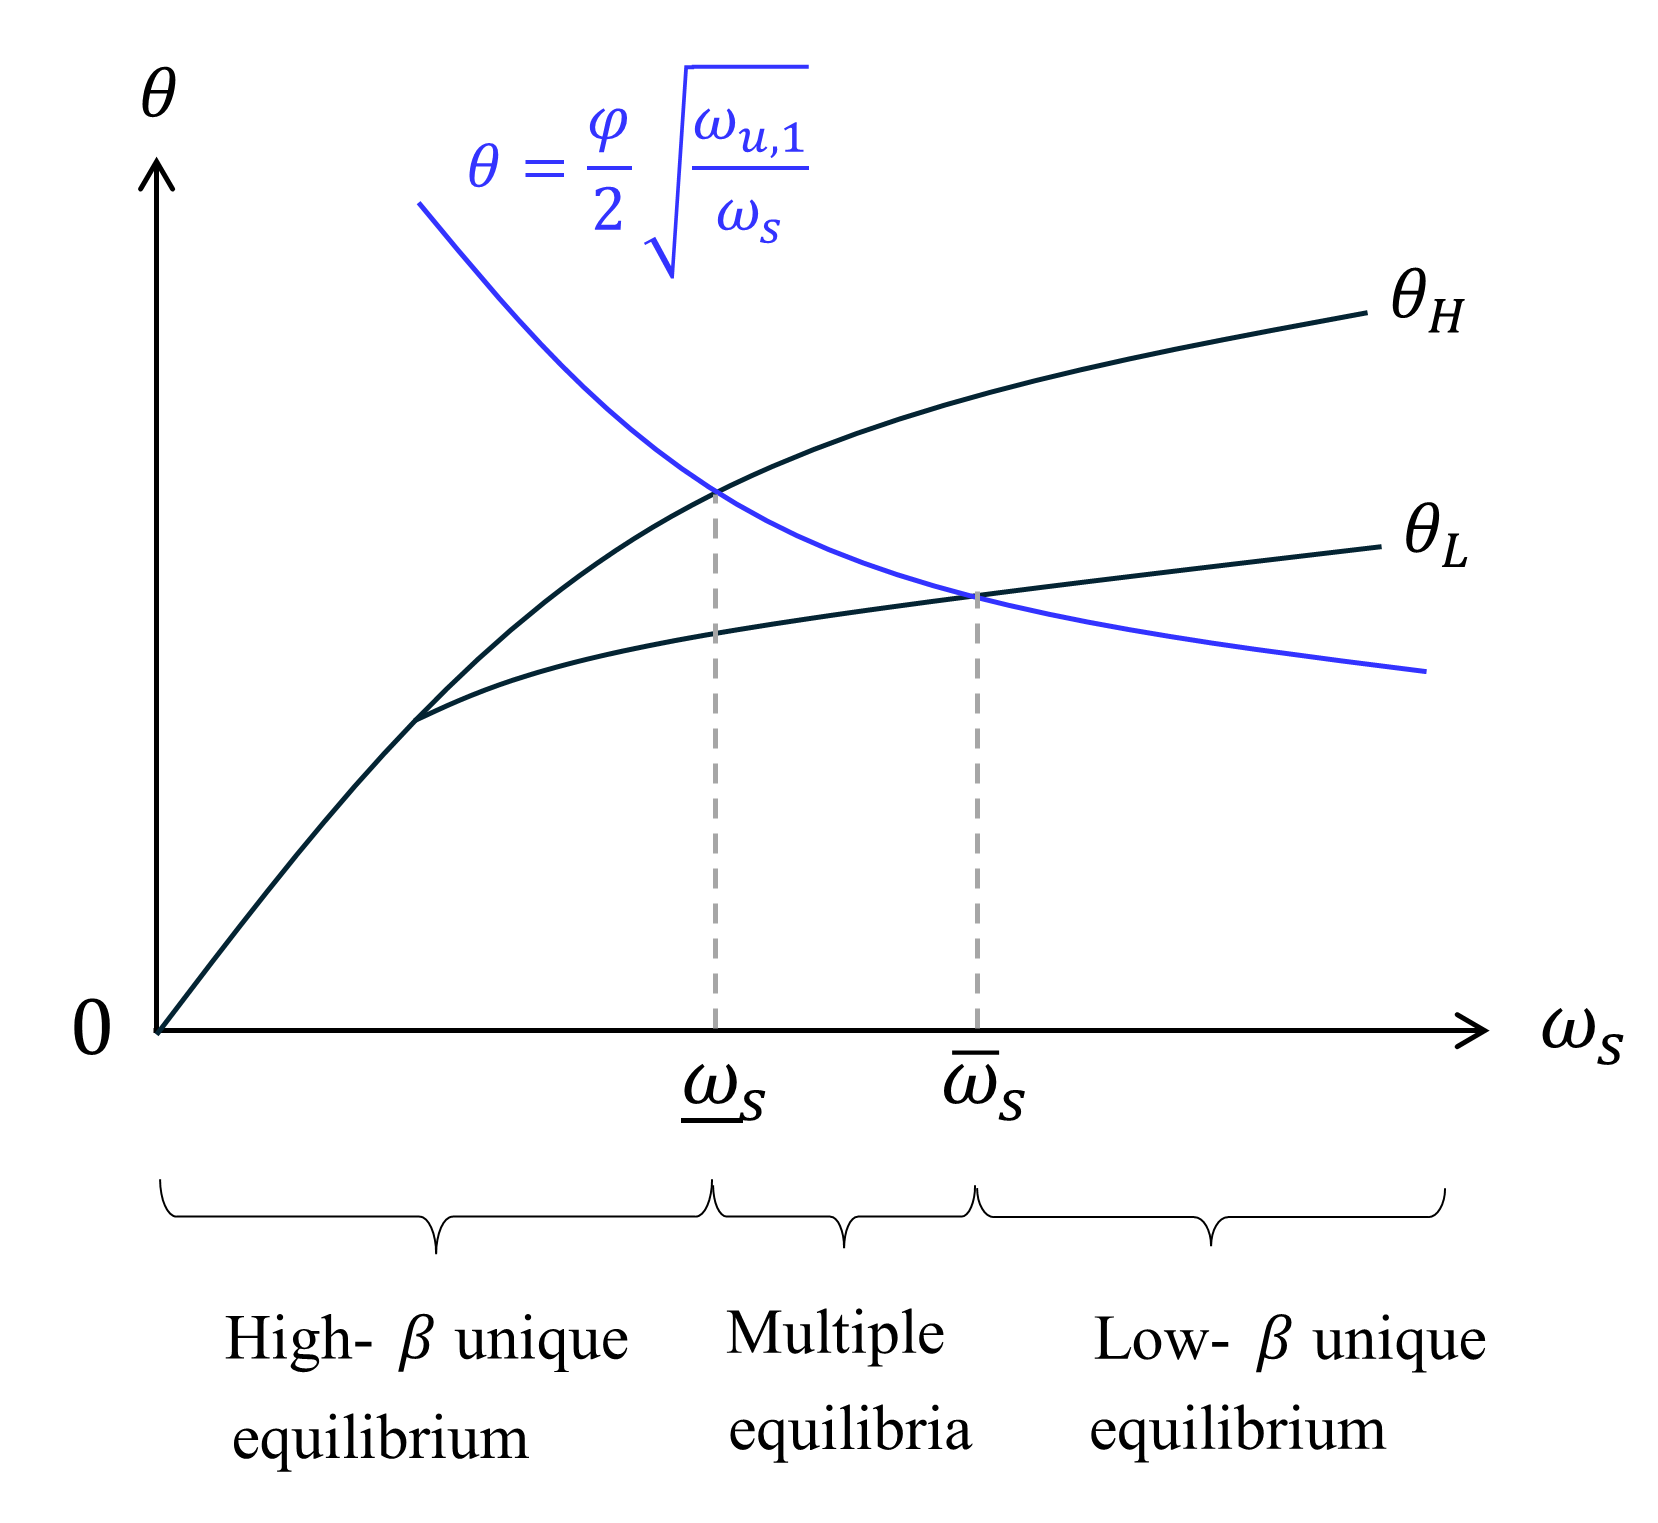
\includegraphics[width=75mm]{./Figures/fig_omegas_theta2.png}
 \label{fig_large_varphi}}
 \subfigure [Small $\varphi$]{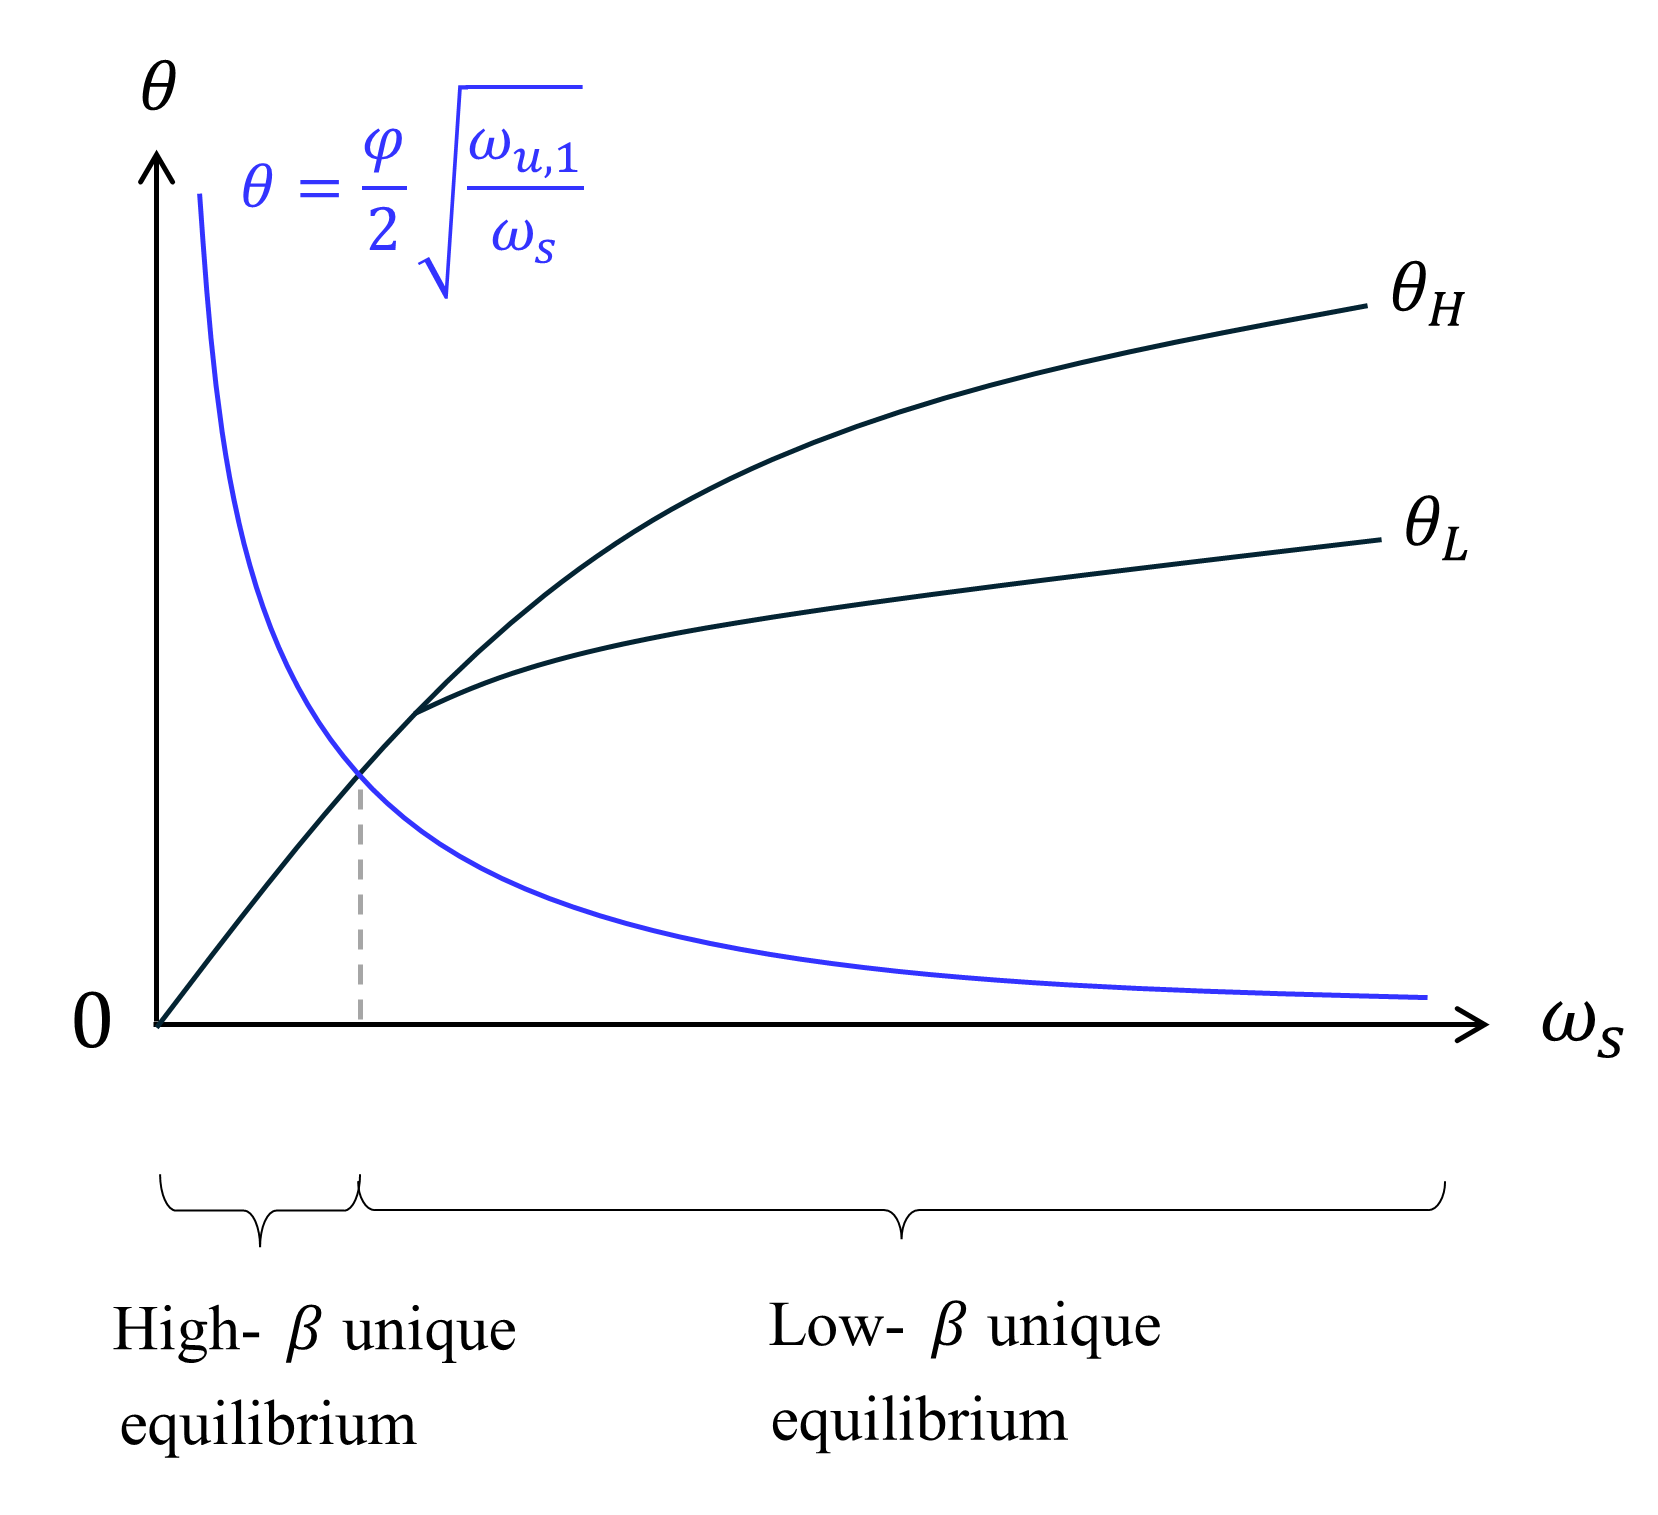
\includegraphics[width=75mm]{./Figures/fig_omegas_theta3.png}\label{fig_small_varphi}}
 \caption{Equilibrium Characterization with Endogenous $\theta$}
 \caption*{\footnotesize{Note: These figures illustrate the equilibrium states using the reputation concern, $\theta$, and the skill potential, $\omega_{s}$. The curves represented by $\theta_{H}$ and $\theta_{L}$ are identical to those in Figure \ref{fig:theta}} and Proposition \ref{prop:eqm}, while $\theta$ is endogenous and decreasing in $\omega_{s}$ as equation (\ref{eq:theta}) suggests.}
     \label{fig:theta_end}
\end{figure}

%\begin{proposition}[Equilibrium in $t=0$]\label{prop:endogenous}
%In $t=0$, there are two thresholds of the skill potential, denoted as $\ubar{\omega}_{s}>0$ and $\bar{\omega}_{s} (\geq \ubar{\omega}_{s})$, such that,
% \begin{enumerate}[label=(\roman*)]
%\item If $\omega_{s} \geq \bar{\omega}_{s}$, then the low-$\beta$ equilibrium uniquely realizes.
%\item If $\omega_{s} \in (\ubar{\omega}_{s}, \bar{\omega}_{s})$, then both the high- and low-$\beta$ equilibria arise.
%\item If $\omega_{s} \leq \ubar{\omega}_{s}$, then the high-$\beta$ equilibrium uniquely realizes.
%\end{enumerate}
%\end{proposition}

Since the trader's reputation concern $\theta$ is endogeneized as \eqref{eq:theta}, which is a decreasing function of $\omega_{s}$, Figure \ref{fig:theta_end} is obtained by overlaying \eqref{eq:theta} on Figure \ref{fig:theta}. The first and the second parts of Proposition \ref{prop:endogenous} correspond to panels (a) and (b) of Figure \ref{fig:theta_end}, respectively. Proposition \ref{prop:endogenous} states that multiple equilibria may arise only when labor mobility is sufficiently high ($\varphi$ is large), i.e., only when the traders have a large reputation concern, $\theta$.\footnote{Equation (\ref{eq:varphi*}) in Online Appendix \ref{proofendogenous} provides the definition of the boundary value of $\varphi$ that classifies cases 1 and 2 in Proposition \ref{prop:endogenous}.} Since the case in panel (a) yields richer implications, while panel (b) is qualitatively similar to \citet{kyle1985continuous}, we focus on the case in panel (a), which arises when $\varphi$ is relatively large.

Panel (a) of Figure \ref{fig:theta_end} shows that, as a result of endogeneizing $\theta$ as a function of $\omega_{s}$, the conditions characterizing the equilibrium types simplify to a single condition solely on $\omega_{s}$: a large $\omega_{s}$ yields a unique low-$\beta$ equilibrium, an intermediate $\omega$ generates multiple equilibria, and a small $\omega_{s}$ leads to a unique high-$\beta$ equilibrium.

%As the trader's reputation concern ($\theta$) decreases with the skill potential, Proposition \ref{prop:eqm} in the baseline model is generalized, and multiple equilibria show up when $\omega_{s}$ is intermediate.\footnote{Numerically, multiple equilibria arise, and three graphs in Figure \ref{fig:exog}  can be replicated when the parameter values are, for example, $\omega_{s}=50$, $\omega_{\delta}=1$, $\omega_{u,0}=0.1$, and $\omega_{u,1}=60$.} Accordingly, Figure \ref{fig:theta_end}, which illustrates Proposition \ref{prop:endogenous}, is obtained by overlaying the downward-sloping curve of $\theta$ defined by equation (\ref{eq:theta}) on Figure \ref{fig:theta}.


The intuition is as follows. When the skill potential is high ($\omega_{s}\geq\bar{\omega}_{s}$), the trader is more likely to have a large informational advantage
over the market maker. This leads to a strong price impact, making it costly to inflate the trading strategy to receive high reputation.
Consequently, she is more inclined to adopt profit-seeking strategies, and the Kyle-like equilibrium is uniquely realized. As the skill potential decreases, however, the trader's informational advantage and the price impact tend to diminish, making it easier to prioritize her reputation concerns. Therefore, for intermediate levels of $\omega_{s} \in(\ubar{\omega}_{s},\bar{\omega}_{s})$, the reputation-driven equilibrium arises and coexists with the Kyle-like equilibrium. If the skill potential declines further ($\omega_{s} \leq \ubar{\omega}_{s}$), the reputation becomes the dominant factor, and the Kyle-like equilibrium disappears.

%===========================================
\subsection{Implications}\label{ss:implications}
This section discusses economic implications drawn from the equilibrium analyses in Section \ref{ss:eqm_endog}.
%-------------------------------------------
%\subsubsection{High-$\beta$ vs. low-$\beta$ equilibrium}
\subsubsection{Skills, Trading Styles, and Financial Fragility}

%-------------------------------------------
%\subsubsection{Financial fragility}
The self-fulfilling nature of multiple equilibria suggests that financial markets may become vulnerable to non-fundamental factors. A shift in investor beliefs alone, without any structural changes, could cause the market to transition from the standard Kyle-like equilibrium to the reputation-driven equilibrium, characterized by high price volatility and poor trading performance.
%\footnote{Even with the parameter values that admit a unique equilibrium, a small parameter shift can lead to a significant jump from one stable equilibrium to another if it pushes the economy into the multiple-equilibrium region.} 
We interpret this phenomenon as a form of \textit{fragility} in financial markets. Our model suggests that fragility may occur when labor mobility is high or demand for skills is high in the finance industry, as these factors heighten traders’ reputation concerns in anticipation of future recruitment opportunities. 

Proposition \ref{prop:endogenous} yields novel implications connecting traders' skills, their trading styles, and financial fragility. First, traders with high skill potential ($\omega_{s} \geq \bar{\omega}_{s}$) adopt low-intensity strategies that minimize market impact, prioritizing profits over reputation, whereas those with low skill potential ($\omega_{s} \leq \ubar{\omega}_{s}$) engage in high-intensity strategies with flashy risk taking, seeking reputation in the industry. The model predicts that these tendencies are more pronounced for traders with very high or very low $\omega_{s}$, as the equilibrium is unique at such levels of $\omega_{s}$ (Proposition \ref{prop:endogenous}). 

These results are somewhat consistent with common observations in the real market. For example, skilled HFT firms, such as Citadel Securities or Virtu Financial, are highly profit-driven and focused on consistent performance, leveraging advanced algorithms and technologies. They employ top talent and have a clear performance-based focus, with reputational benefits being regarded as secondary to profitability.
Similarly, hedge fund managers often vary in their approach depending on their skill level and reputation. Studies show that highly skilled managers, such as those at Bridgewater or Renaissance Technologies, are more focused on generating long-term performance through data-driven strategies (\citealp{schwager2012hedge}). On the other hand, lesser-known funds sometimes take on highly visible and risky bets that generate headlines but do not always result in sustainable returns. The high-profile blowup involving Archegos Capital in 2021 is the leading example that illustrates how traders seeking visibility through concentrated and flashy positions can underperform and may go bankrupt.

%Proposition \ref{prop:endogenous} makes a novel contribution by clarifying the relation between traders' skill potential and financial fragility. Firstly, it indicates that a trader exhibits distinctive trading activity according to her skill potential, which is more pronounced and observable when she is equipped with low or high skill potential due to the uniqueness of the equilibrium. Namely, traders with high skill potential ($\omega_{s} \geq \bar{\omega}_{s}$) tend to trade at the performance-maximizing level, meaning that their $\beta$ is close to the \citet{kyle1985continuous} equilibrium. On the other hand, traders with low skill potential ($\omega_{s} \leq \ubar{\omega}_{s}$) engage in more flashy risk trading by inflating $\beta$ far away from the performance-maximizing level just to corroborate their reputation. 

%The above result supports somewhat common observations in the real market. For example, skilled HFT firms, such as Citadel Securities or Virtu Financial, are highly profit-driven and focused on consistent performance, leveraging advanced algorithms and technologies. These firms employ top talent and have a clear performance-based focus, with reputational benefits being regarded as secondary to profitability. Similarly, hedge fund managers often vary in their approach depending on their skill level and reputation. Studies show that highly skilled managers, such as those at Bridgewater or Renaissance Technologies, are more focused on generating long-term performance through data-driven strategies (\citealp{schwager2012hedge}). On the other hand, lesser-known funds sometimes take on highly visible and risky bets that generate headlines but do not always result in sustainable returns. The high-profile blowup involving Archegos Capital in 2021 is the leading example that illustrates how traders seeking visibility through concentrated and flashy positions can underperform and may go bankrupt.

The second implication is drawn from the model's multiple equilibria. Namely, the relation between traders' activities and skills may become blurry when their skill potential is mediocre ($\omega_{s}\in (\ubar{\omega}_{s}, \bar{\omega}_{s}$)). Notably, this indeterminacy may lead to financial fragility. Depending on market beliefs, intermediate-skilled traders may shift between profit-seeking and reputation-driven strategies, creating non-fundamental fluctuations. Our result suggests that even relatively skilled traders may follow the crowd due to market beliefs, hopping between safe and risky strategies. 

A notable observation in line with this result is momentum crashes (\citealp{daniel2016momentum}), where traders engaging in risky and visible momentum trades often switch to safer strategies, generating sharp reversals and amplifying price declines. More generally, the rapid shifts between risk-taking and solid performance-based behavior have contributed to market fragility and volatility, as documented in various studies on economic crises, such as \citet{brunnermeier2009deciphering} on the credit crunch during the Global Financial Crisis in 2007. Importantly, large fundamental shifts that support such transitions are rarely identified (\citealp{gennotte1999market}). Our model does not require such fundamental shocks, as a mere change in beliefs can trigger a shift.

%Secondly, Proposition \ref{prop:endogenous} implies that the relationship between the trading activity and the underlying skill potential becomes more blurry when traders have intermediate skill potentials ($\omega_{s}\in (\ubar{\omega}_{s}, \bar{\omega}_{s}$)). Notably, this indeterminacy leads to financial fragility. Depending on market beliefs, intermediate-skilled traders exhibit multiple equilibria and can shift between profit-driven and reputation-driven strategies, creating non-fundamental fluctuations. Our result suggests that even relatively skilled traders may follow the crowd due to market beliefs, hopping between safe and risky strategies. A notable observation in line with this result is momentum crashes (\citealp{daniel2016momentum}), where traders engaging in risky and visible momentum trades often switch to safer strategies, generating sharp reversals and amplifying price declines. More generally, the rapid shifts between risk-taking and solid performance-based behavior have contributed to market fragility and volatility, as documented in various studies on economic crises, such as \citet{brunnermeier2009deciphering} on the credit crunch during the Global Financial Crisis in 2007. Importantly, large fundamental shifts that support such transitions are rarely identified (\citealp{gennotte1999market}). Our model does not require such fundamental shocks, as a mere change in beliefs can trigger a shift.


%===========================================
\subsubsection{Compensation in Finance Industry} \label{sss:wages}
\begin{figure}
\centering
{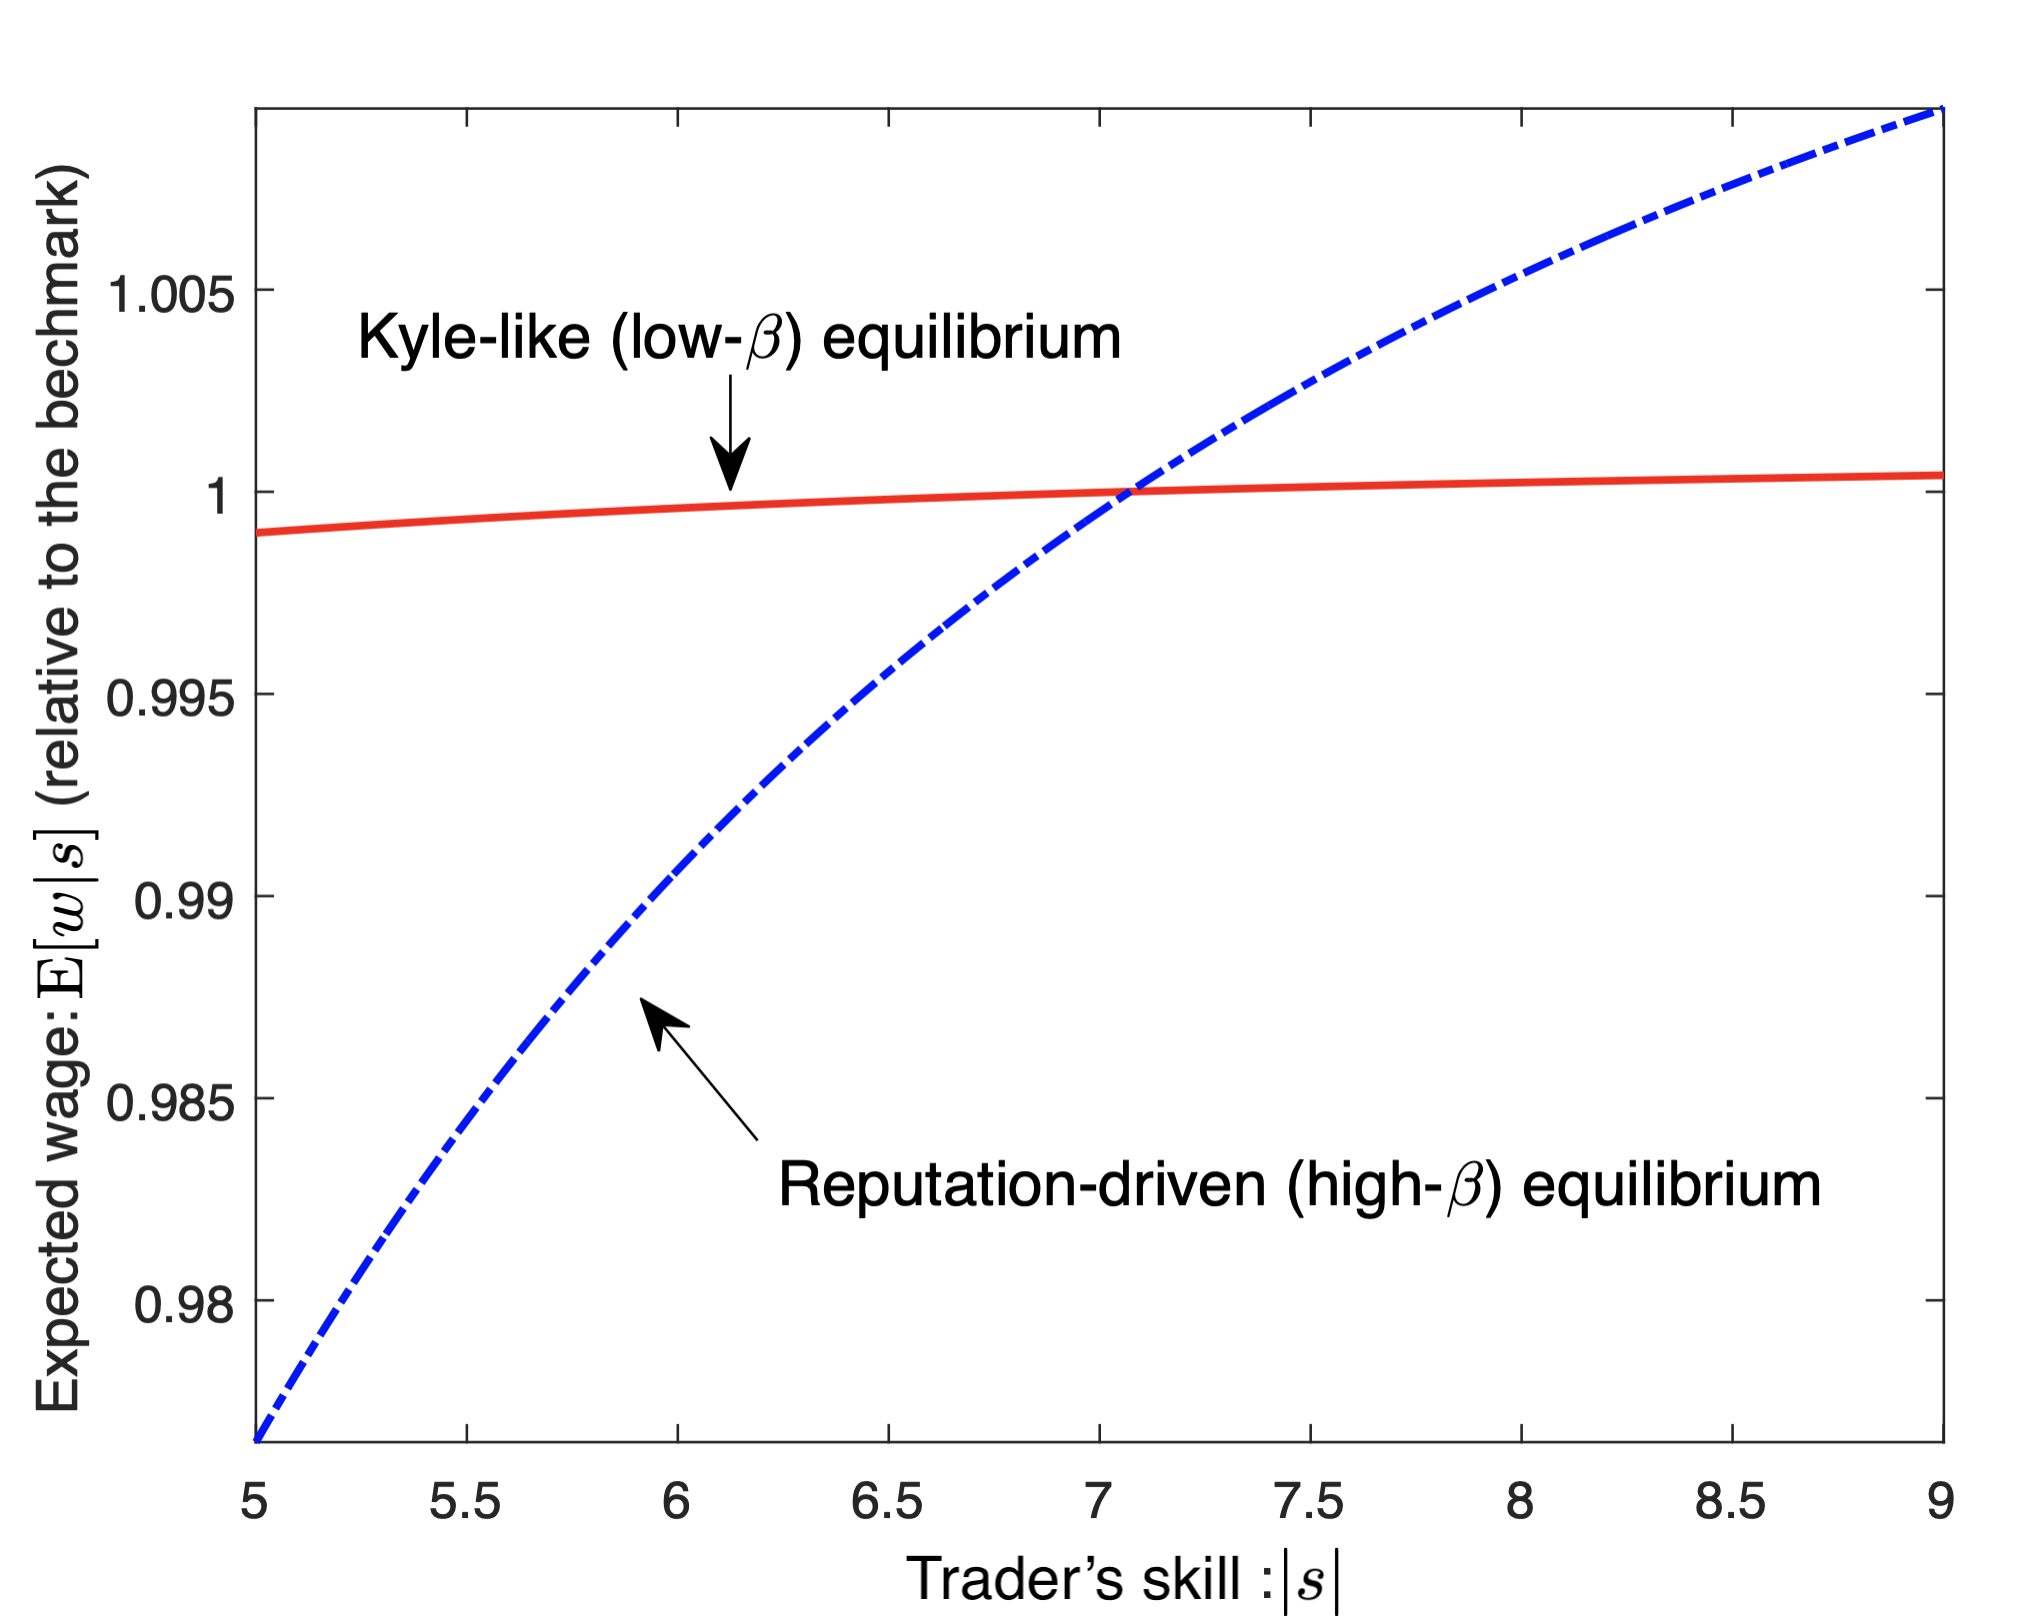
\includegraphics[width=80mm]{./Figures/RelativeWages3.png}}
\caption{Skill versus Expected Wage}
\caption*{\footnotesize{Note: The figure plots the trader's expected wages (relative to the benchmark with $\theta=0$) at the low-$\beta$ equilibrium (solid line) and high-$\beta$ equilibrium (dashed line) for different levels of skill, $|s|$. The parameter values used in the figures are $\omega_{s}=50$, $\omega_{\delta}=1$, $\omega_{u,0}=0.1$, $\omega_{u,1}=60$, and $\theta=\frac{\varphi\beta_1}{2}\approx0.33$ ($\varphi=0.6$).}}\label{fig:wageSens}
\end{figure}

Our model provides insights into how skills are reflected in compensation in the financial industry. As shown in statement \ref{item:5} of Corollary \ref{cor:high_vs_low}, the recruiter learns $s$ more precisely in the high-$\beta$ equilibrium than in the low-$\beta$ equilibrium, as the trader demonstrates her skill by trading more intensively. Consequently, traders' wages become more sensitive to their skills. As an illustration, Figure \ref{fig:wageSens} plots the traders' expected wages in relation to their skills in the low- and high-$\beta$ equilibria. In the high-$\beta$ equilibrium, the recruiter's accurate evaluations result in greater pay inequality: low-skilled ones receive very low wages, while high-skilled ones are very highly paid. This result corroborates empirical observations, such as those provided by \citet{philippon2012wages} and \citet*{bohm2018since}, highlighting the comparatively large wage inequality in the finance industry. \citet{celerier2019returns} attribute its source to the scalability of skill, while inequality arises from traders' reputation concerns in our model. %{\color{red}[TO REWRITE]}

%\begin{figure}
%\centering
%{\includegraphics[width=90mm]{PercRatios2.pdf}}\\[10pt]
%\caption{Equilibrium pay inequality. The figure plots the 97--3, 90--10, and 50--10 expected wage percentile ratios at the high-$\beta$ equilibrium (hatched), low-$\beta$ equilibrium (cross-hatched), and benchmark, $\theta=0$, equilibrium (unhatched). The parameter values used in the figure are $\theta=\frac{\varphi\beta_{1}}{2}=0.33$, $\sigma^{2}_{s}=50$, $\omega_{\delta}=1$, and $\sigma_{0,u}^{2}=0.1$.}\label{fig:ineq}
%\end{figure}
%% or diagonal hatch lines, criss-cross hatch lines

%Moreover, higher returns to skill in the reputation-driven equilibrium lead to greater pay inequality among high- and low-skilled traders. This result corroborates empirical observations, such as those provided by \citet{philippon2012wages} and \citet*{bohm2018since}, highlighting the comparatively large wage inequality in the finance industry. \citet{celerier2019returns} attribute its source to the scalability of skill, while inequality arises from traders' reputation concerns in our model.
%\bigskip
%\centerline{\bf [Place Figure~\ref{fig_endogenous} about here]}
%\bigskip

Our results also have implications for the wage structure in the finance industry. The model suggests that moving away from performance-tied compensation and assigning more weight to the fixed salary component creates reputation concerns, thereby generating fragility in financial markets. Recall that reputation concerns stem from the dependence of future salaries on current trading, as the recruiter learns about skill from the realized execution prices. Suppose instead that after meeting a trader, the recruiter hires her for a salary that depends entirely on  $t=1$ trading performance. Since trading actions at $t=0$ bear no consequence on trading profits at $t=1$, the trader's objective at $t=0$ is only to maximize her short-run profits. That is, traders have no reputation concerns, and the model collapses to the \citet{kyle1985continuous} equilibrium. Therefore, our results highlight the importance of traders' forward-looking motivations—stemming from labor mobility within the finance industry—in contributing to financial fragility or pay inequality.

%-------------------------------------------
\subsubsection{Skill and Performance Persistence}

Do high-skilled traders consistently perform well? Not always: skilled traders may not necessarily outperform less skilled ones due to multiple equilibria. Consider a highly skilled trader and a relatively less skilled one. Since trading profits are increasing in traders' skill, $|s|$, the former is expected to achieve higher trading profits than the latter \emph{conditional on} both traders trading at the same intensity, $\beta$. However, if the recruiter believes, for whatever reason, that the skilled trader trades more aggressively than the less skilled one, and traders conform to his belief, a high skill level does not translate into performance. This is because the skilled trader, trading at the reputation-driven equilibrium, reveals too much private information to the market maker. Hence, compared to the less skilled trader, who plays the Kyle-like equilibrium, the skilled trader may earn lower expected profits. Figure \ref{fig:perf}  illustrates such a situation. It plots the expected trading profits at high- and low-$\beta$ equilibria with different levels of skill, suggesting that a low-skilled trader in the low-$\beta$ equilibrium (point B) outperforms a high-skill trader in the high-$\beta$ equilibrium (point A).

\begin{figure}
\centering
{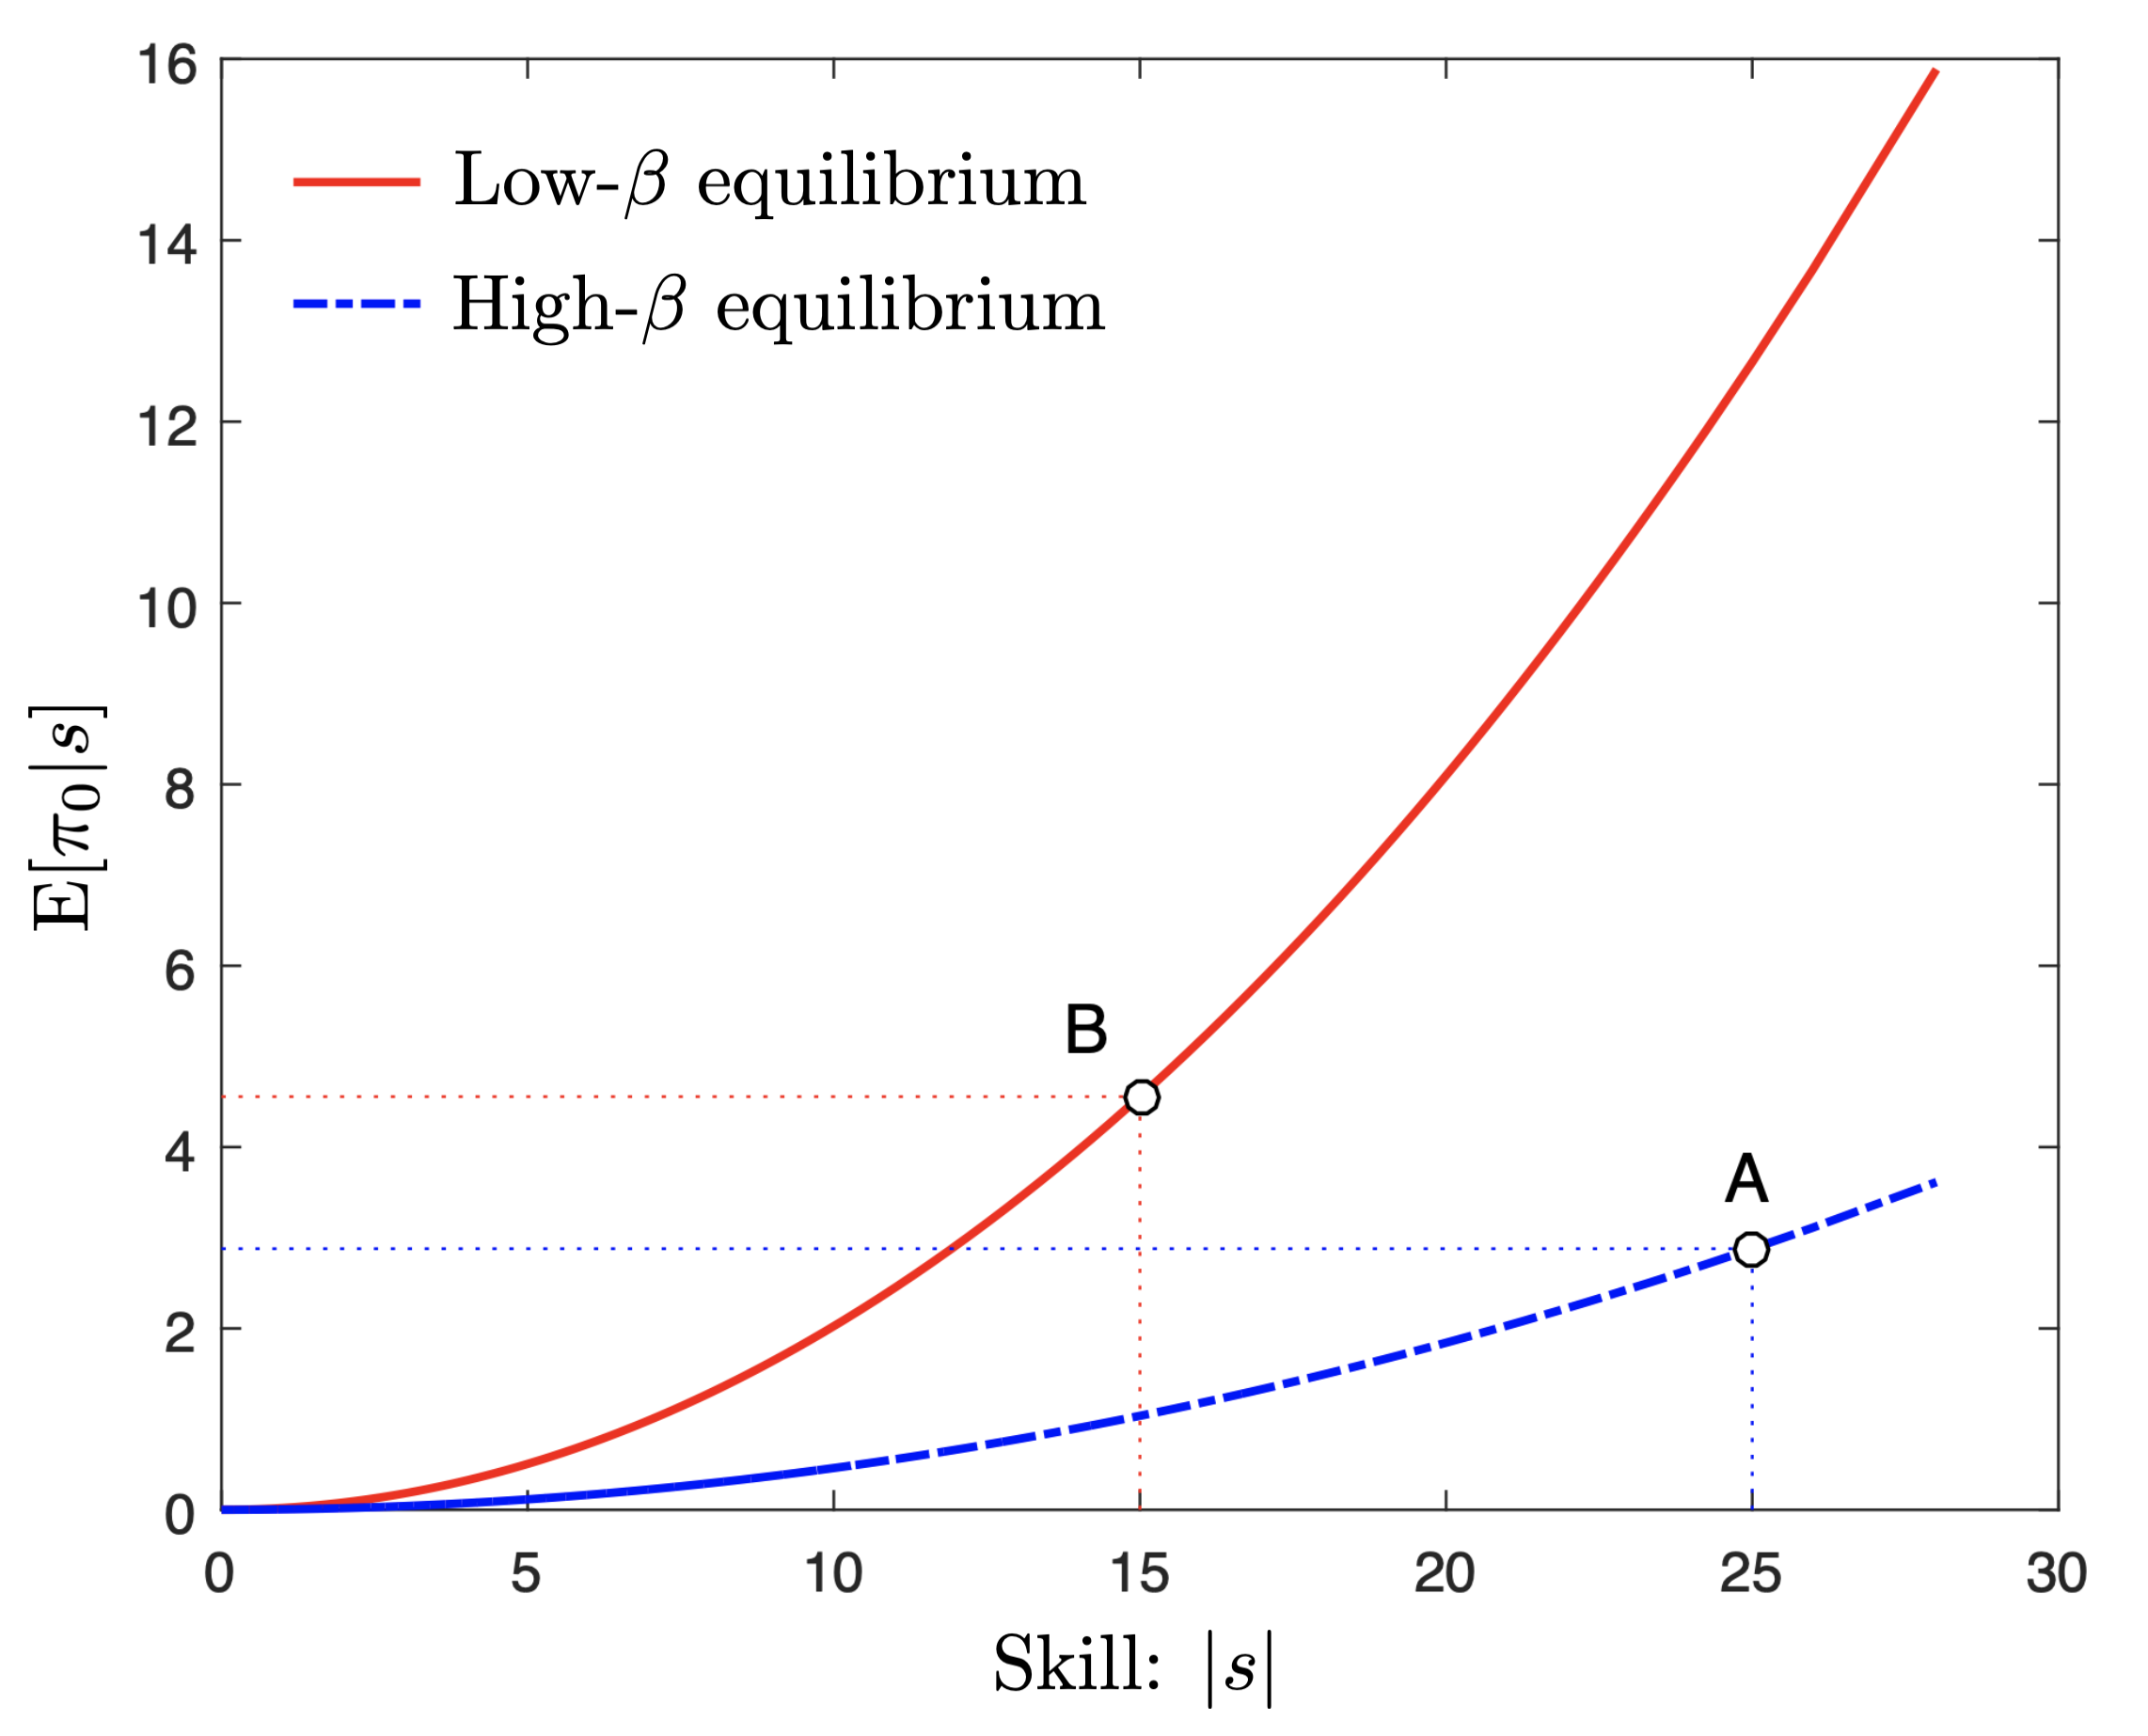
\includegraphics[width=85mm]{./Figures/Performance_s.png}\label{high}}
\caption{Skill versus Expected Trading Profit}
\caption*{\footnotesize{Note: The figure plots the expected trading profit $\mathrm{E}[\pi_{0}|s]$ at the low-$\beta$ equilibrium (solid line) and the high-$\beta$ equilibrium (dashed line) for different levels of skill,  $|s|$. The parameter values used in the figure are $\omega_{s}=50$, $\omega_{\delta}=1$, $\omega_{u}=0.1$, and $\theta=\frac{\varphi\beta_1}{2}\approx0.33$ ($\varphi=0.6$).}}
\label{fig:perf}
\end{figure}

%The empirical literature uses mutual fund data to investigate skill in the finance industry. The results are somewhat mixed. Some papers interpret the lack of performance as measured by the excess return over (passive) benchmarks as lack of skill (see ... papers, Jensen 1967; Busse, Goyal, and Wahal 2010---check that latter claims it means no skill). There are also papers that try to reconcile the lack of performance over the benchmark and per 

The empirical literature (e.g., \citealp{jensen1967performance}; \citealp*{busse2010performance}) finds that asset managers do not outperform passive benchmarks on average and, in cross-section, those who outperform cannot do so consistently. While the literature attributes the lack of persistent performance to the lack of skill, our result proposes an alternative explanation. Several studies reconcile the existence of skill with the lack of persistent performance. \citet{berk2004mutual}, for example, argue that skill-based alphas eventually disappear due to competition between investors and decreasing returns to scale at the fund level.\footnote{\citet*{pastor2015scale} document increases in skill in finance and attribute the lack of corresponding increases in performance to decreasing returns to scale at the industry level.} Our model contributes to the understanding of this matter by showing that the lack of interplay between trader performance and skill could be the result of self-fulfilling multiple equilibria. 
%%*=*=*=*=*=*=*=*=*=*=*=*=*=*=*=*=*=*=*=*=*=*
%\section{Robustness} \label{sec:robust}
%
%We have assumed thus far that the recruiter learns about skill from the price and payoff of the asset picked by the trader. We now show that fragility still obtains when the recruiter uses different sources of information. In particular, we assume that the recruiter observes the profit per unit traded, $\delta-p$, and a noisy signal of the trader's trade, $x+\nu$, where $\nu$ is normal with mean 0 and variance $\sigma_{\nu}^2$. 
%
%(Figure displays the case of multiple equilibria in the determination of beta.) In the high-$\beta$ equilibrium, the trader trades more aggressively that in Kyle (1985). In the low-$\beta$ equilibrium, however, she trades less aggressively. The intuition behind this result is the following. The recruiter learns from two signals that respond in different ways to the trader's order: trading aggressiveness positively affects the noisy trade, but negatively affects the per unit profit, through the positive effect on price. The potential overall effect on reputation may be then ambiguous. Note that the effect of trading on reputation is similar to the effect of trading on profits: price impact is higher, making the profit per unit traded lower, but with more units traded the overall profit may increase. %Fragility obtains because the recruiter learns from two sources of information.